In~\cite{Weghe2007}, the TM framework for crisp intervals is introduced, based on~\cite{Kulpa1997}. In~\cite{DeTre2012}, the framework is generalized to allow the representation of and reasoning with time intervals subject to uncertainty. In this section, this generalization's main aspects towards interval representation and Allen relationship evaluation are briefly presented. 

\subsection{\label{subsec:tm-preliminaries}Preliminary Concepts}
In the triangular model framework, the approaches to interval representation and Allen relationship evaluation are closely related to the approach to interval visualization. Usually, different time intervals are visualized as different parallel line segments in the same image plane. However, as this linear approach introduces a few issues, time intervals are visualized as points in the image plane in the TM framework~\cite{DeTre2012},~\cite{Weghe2007}. To achieve this, a horizontal line segment visualizing the used (part of the) time axis is drawn in the image plane (this is called the \emph{time line}). Then, a triangle is drawn, using this line segment as a side of which the angles with the other two sides have sizes $\alpha$ and $-\alpha$ respectively. The area contained in this triangle is called the \emph{interval space} and will contain all visualizations of intervals. Now, the procedure used to visualize a CTI $\left[s, e\right]$ in the interval space is the following~\cite{DeTre2012},~\cite{Weghe2007}:
\vspace{-5pt}
\begin{enumerate}
	\item $s$ is visualized as a point on the time line.
	\item A straight half-line $L_s$ is constructed from this point, having, in this point, an angle of size $\alpha$ with the time line.
	\item $e$ is visualized as a point on the time line.
	\item A straight half-line $L_e$ is constructed from this point, having, in this point, an angle of size $-\alpha$ with the time line.
	\item The intersection point of $L_s$ and $L_e$ is the intended visualization of interval $\left[s, e\right]$.
\end{enumerate}
\vspace{-5pt}
A similar point visualizing an interval is generally called an \emph{interval point}~\cite{DeTre2012},~\cite{Weghe2007}. In this work, as it is usually done, the size of $\alpha$ is chosen to be $45^{\circ}$. An example of such construction is shown in figure \ref{fig:tm-const-ex}.

\begin{figure}[h]
	\centering
	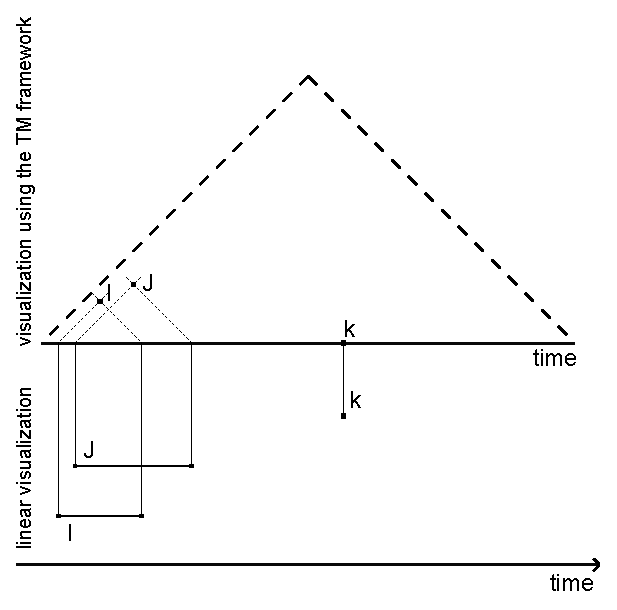
\includegraphics[width=0.9\columnwidth]{graphs/TM_model_several.eps}
	\caption{The visualization of several CTI using the TM framework.}
	\label{fig:tm-const-ex}
\end{figure}
\vspace{-10pt}

\subsection{\label{subsec:tm-interval}Representation of Time Intervals Subject to Uncertainty}
The TM framework allows uncertainty in time intervals by supporting uncertain time intervals~\cite{DeTre2012}:

\begin{definition}
Given an ordered set of instants $T$, an \emph{uncertain time interval} (UTI) $J$ in $T$ is here a time interval defined by a pair
\begin{align}
J \triangleq (\pi_s, \pi_e) \nonumber
\end{align}
where $\pi_s$ and $\pi_e$ are two convex~\cite{Dubois1983} possibility distributions on $T$.
\end{definition}

Consider an ordered set of instants $T$ and an UTI $J$ in $T$, defined by the pair $(\pi_s, \pi_e)$. Given an instant $x \in T$, $\pi_s(x)$ now expresses the possibility that $x$ is the starting instant of $J$ and $\pi_e(x)$ expresses the possibility that $x$ is the ending instant of $J$. Thus, $J$ intends to indicate just one CTI, but it is (partially) unknown exactly which time interval this is. The possibility $\pi_J(I)$ that a given CTI $I = \left[s_i, e_i\right]$ is the exact time interval intended by $J$ can now be uniquely determined by~\cite{DeTre2012}:
\vspace{-5pt}
\begin{align}
\pi_J(I) = \begin{cases}
 \min \left(\pi_s (s_i), \pi_e (e_i) \right), & \mbox{ if } s_i \leq e_i\\
0, & \mbox{ otherwise }
\end{cases}
\end{align}

Now consider an ordered set of instants $T$ and a visualization of this in an image plane, using the TM framework. An UTI $J$ in $T$ defined by a pair $(\pi_s, \pi_e)$ is now visualized as an area in the image plane. This area is constructed as follows: for every CTI $K$ for which the possibility $\pi_J(K)$ of $K$ being the CTI intended by $J$ is higher than zero, the interval point is drawn and is given a color. This color is part of a linear single-color greyscale and its saturation is linearly related to the degree of possibility that $K$ is the CTI intended by $J$. Together, these drawn interval points form the visualization of $J$~\cite{DeTre2012}. An example of such construction is shown in figure \ref{fig:tm-ill-const-ex}. In this figure, a darker color of interval point indicates a higher and a lighter color a lower possibility that the corresponding CTI is the intended interval.

\begin{figure}[h]
	\centering
	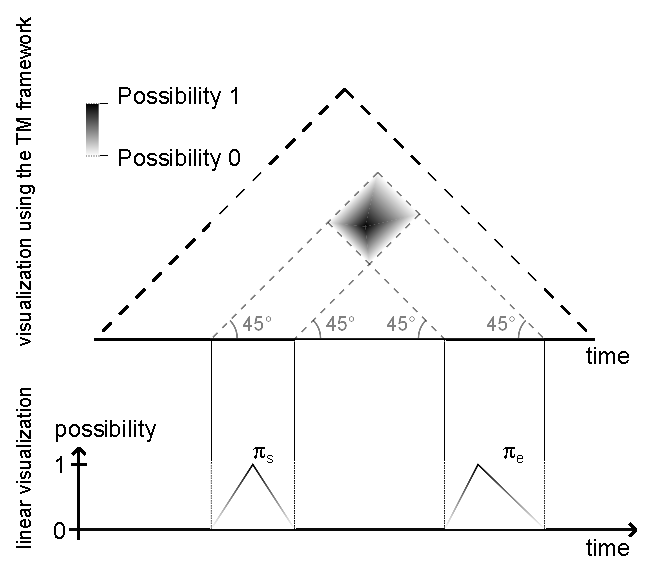
\includegraphics[width=0.9\columnwidth]{graphs/TM_model_ill_known.eps}
	\caption{The visualization of one UTI defined by a pair $(\pi_s, \pi_e)$ using the TM framework.}
	\label{fig:tm-ill-const-ex}
\end{figure}
\vspace{-10pt}

\subsection{\label{subsec:tm-evaluation}Evaluation of Allen Relationships}
At the base of the framework's approach to evaluating Allen relationships is the concept of uncertain relational zones~\cite{DeTre2012}:

\begin{definition}
For a given UTI $J$, the \emph{uncertain relational zones} (URZ) are fixed areas in the interval space.
\end{definition}

Now, given an UTI $J$ and its visualization in an interval space, the procedure to visualize its URZ is the following~\cite{DeTre2012}:

\begin{enumerate}
	\item The visualizations (the points) on the time line of both the smallest and greatest instant with a non-zero possibility of being the starting instant of $J$ are determined.
	\item Two straight half-lines are constructed from each of these points: one having, in the point, an angle of size $\alpha$ with the time line and one having, in the point, an angle of size $-\alpha$ with the time line.
	\item The visualizations (the points) on the time line of both the smallest and greatest instant with a non-zero possibility of being the ending instant of $J$ are determined.
	\item Two straight half-lines are constructed from each of these points: one having, in the point, an angle of size $\alpha$ with the time line and one having, in the point, an angle of size $-\alpha$ with the time line.
	\item The lines constructed this way divide the interval space in at most fifteen different areas, including the area corresponding to the visualization of $J$ itself. These areas are the intended visualizations of $J$'s URZ.
\end{enumerate}

In this procedure, $\alpha$ is the same angle size as in the procedure for the visualization of CTI. The results of this procedure for an example UTI $J$ (as wel as the visualization of $J$ itself) are shown in figure \ref{fig:tm-urz}. 

\begin{figure}[h]
	\centering
	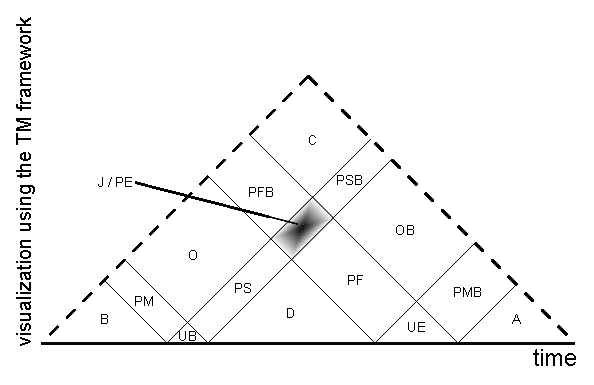
\includegraphics[width=0.9\columnwidth]{graphs/TM_model_URZ.eps}
	\caption{The visualization of the URZ for a given UTI $J$, using the TM framework.}
	\label{fig:tm-urz}
\end{figure}

Given an UTI $J$ and its URZ, every URZ is assigned a symbol and a name and corresponds to a set of Allen relationships~\cite{DeTre2012}. These symbols and names are used to uniquely identify each of $J$'s URZ. The set of Allen relationships corresponding to an URZ contains every Allen relationship in which any interval visualized by one of the URZ's interval points could be with the interval intended by $J$, depending on exactly which CTI $J$ actually intends to represent. In figure \ref{fig:tm-urz}, the URZ's symbols are noted inside the areas visualizing their respective URZ's. In table \ref{tab:urz}, every different row corresponds to a different URZ. In the first two columns, the symbol and name of the URZ are given, the last column contains the set of corresponding Allen relationships. For these, the following notations are used:

\begin{itemize}
	\item `E' denotes `equals'.
	\item `S' denotes `starts'.
	\item `SB' denotes `started by'.
	\item `F' denotes `finishes'.
	\item `FB' denotes `finished by'.
	\item `M' denotes `meets'.
	\item `MB' denotes `met by'.
	\item `O' denotes `overlaps'.
	\item `OB' denotes `overlapped by'.
	\item `D' denotes `during'.
	\item `C' denotes `contains'.
	\item `B' denotes `before'.
	\item `A' denotes `after'.
\end{itemize}
\vspace{-10pt}
\begin{table}[h]
\centering
\begin{tabular}{|l|l|l|}
\hline
Symbol & Name & Relationships \\
\hline
B    & Before & B \\
O    & Overlaps & O \\
C    & Contains & C \\
D    & During & D \\
OB   & Overlapped By & OB \\
A    & After & A \\
PM   & Possibly Meets & M, B, O \\
PS   & Possibly Starts & O, S, D \\
PFB  & Possibly Finished By & O, FB, C \\
\multirow{2}{*}
{PE}   & Possibly Equal  & E, FB, SB, F,\\
       &                 & S, C, D,O, OB \\
PSB  & Possibly Started By & C, OB, SB \\
PF   & Possibly Finishes & OB, F, D \\
PMB  & Possibly Met By & OB, MB A \\
UB   & Uncertain Beginning & B, M, O, S, D \\
UE   & Uncertain Ending & D, F, OB, MB, A \\
\hline
\end{tabular}
\caption{The fifteen possible URZ for a given UTI.}
\label{tab:urz}
\end{table}
\vspace{-5pt}
The TM framework now allows evaluating the Allen relationships a given CTI $I = \left[s, e\right]$ could be in with a given UTI $J$, depending on the exact CTI intended by $J$. This is done as follows. First, $J$ and its URZ are visualized in an interval space. Next, $I$'s interval point, its construction half-lines $L_s$ and $L_e$ and the visualization of its starting and ending instants on the time line are drawn in the same interval space. Then, evaluation is a matter of position (in the following, the possibility that $I$ is the interval intended by $J$ is denoted $\pi_J(I)$ and the possibility that $I$ is in Allen relationship $AR$ with $J$ is denoted  $\Pos(I\ AR\ J)$)~\cite{DeTre2012}:
\vspace{-5pt}
\begin{itemize}
	\item if $I$'s interval point is located in an URZ corresponding with a singleton of Allen relationships $\{R\}$, it is in relationship $R$ with the interval intended by $J$, whichever this interval is. Thus: $\Pos(I\ AR\ J) = 1$.
	\item if $I$'s interval point is located in an URZ corresponding to a non-singleton set of $n$ Allen relationships $\{R_1, R_2, \ldots, R_n\}$, two more half-lines are drawn: one (denoted $L_s'$) from the visualization of $s$ on the time line, having, in this point, an angle of size $-\alpha$ with the time line and one (denoted $L_e'$) from the visualization of $e$ on the time line, having, in this point, an angle of size $\alpha$ with the time line. Now, some of these half-lines $L_s$, $L_s'$, $L_e$ and $L_e'$ may intersect with the area visualizing $J$. These intersection line segments will divide the area visualizing $J$ in $n$ area parts $p_i, 1 \leq i \leq n$ (intersection line segments also count as area parts), each containing only interval points visualizing intervals with a non-zero possibility of being the interval intended by $J$. Each of these parts $p_i$ will now correspond to an Allen relationship $R_i$. Now, for each $R_i$:
	\begin{equation}
		\Pos(I\ R_i\ J) = \sup_{K \in p_i} \pi_J(K)
	\end{equation}
\end{itemize}

Here, the intervals $K$ are CTI and the expression `$K \in p_i$' is a notation to express that $K$ is visualized by an interval point contained in area part $p_i$.
